\begin{frame}{Image Representation}
\begin{figure}
    \centering
    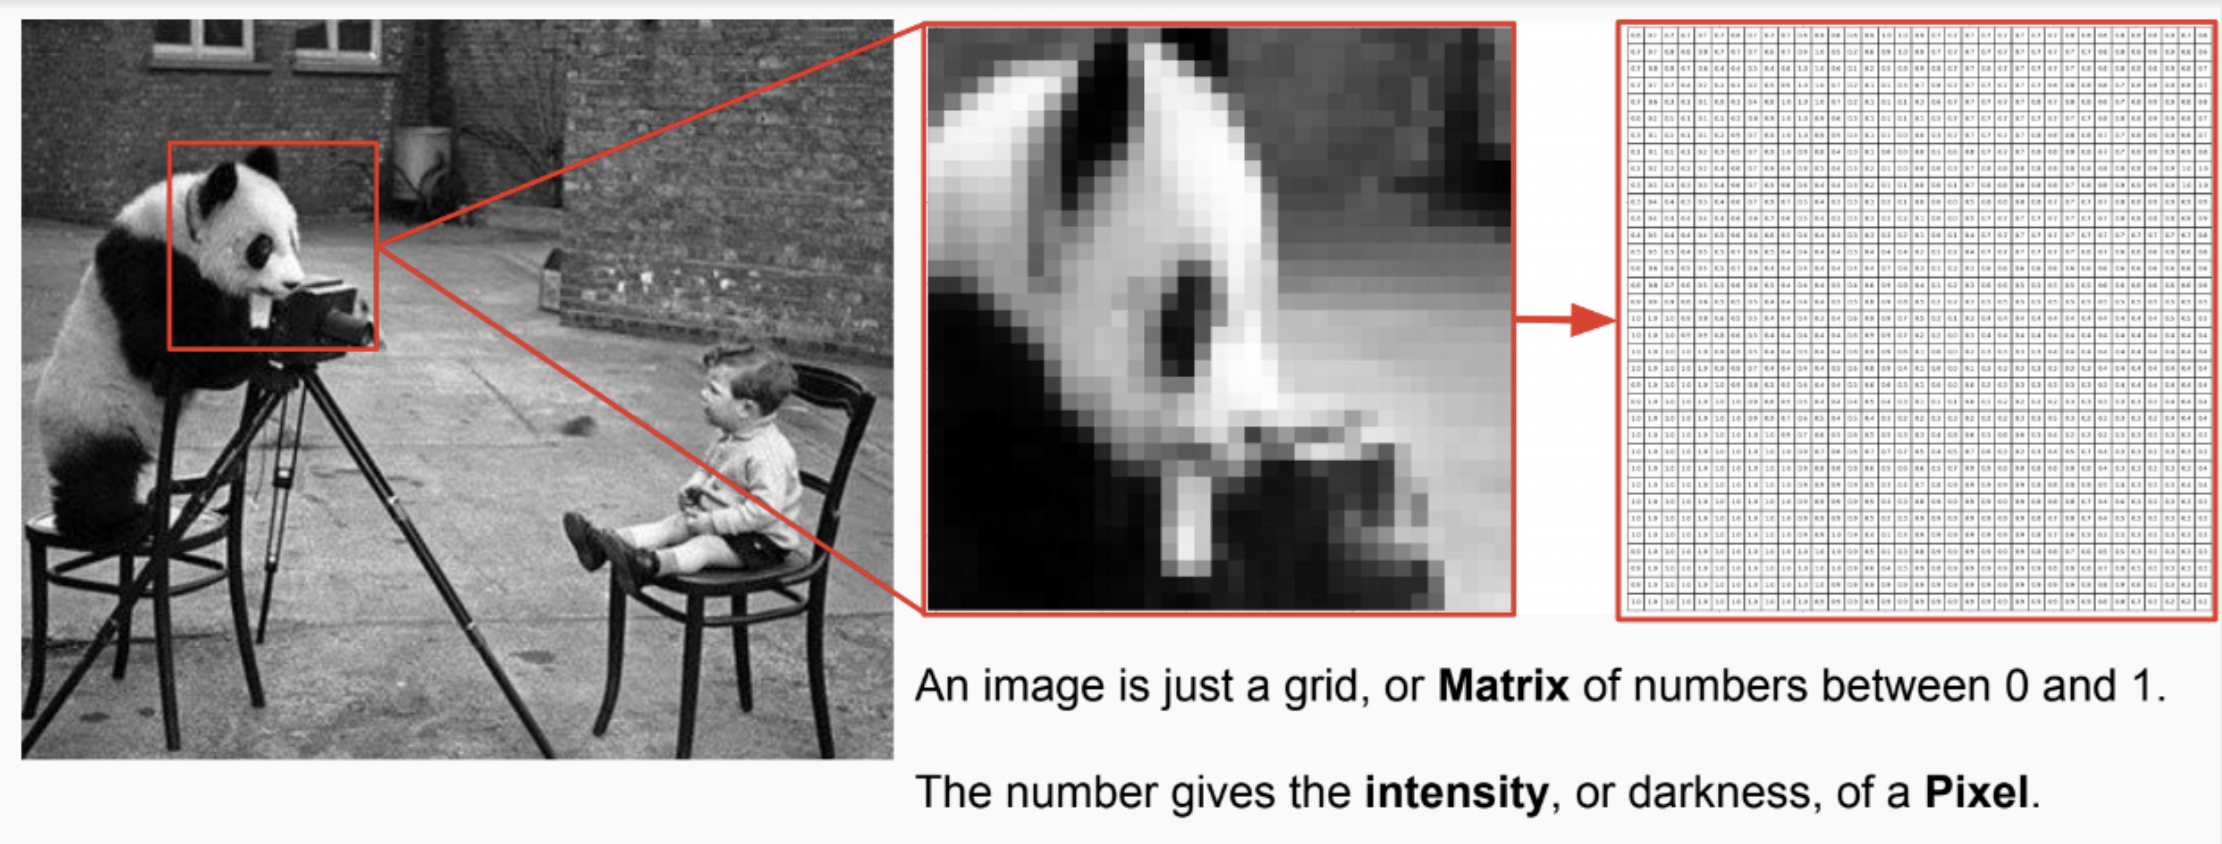
\includegraphics[width=0.9\textwidth]{img/greyscaleimage.png}
    \caption{Black \& White image of panda is a matrix}
\end{figure}
\end{frame}

\begin{frame}{Representing Color}
\begin{figure}
    \centering
    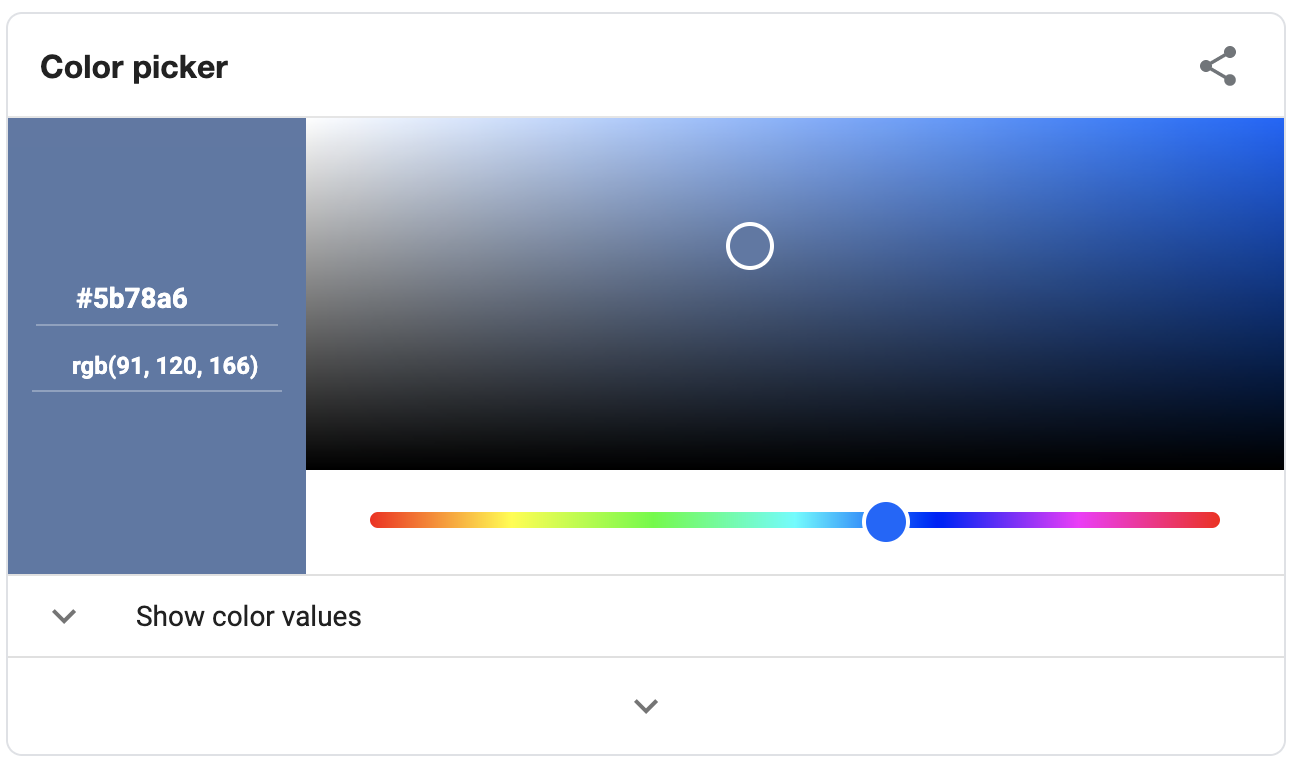
\includegraphics[width=0.9\textwidth]{img/colorpicker.png}
    \caption{Color of single pixel is represented by combination of 3 RGB values}
\end{figure}
\end{frame}

\begin{frame}{Representing Color}
\begin{figure}
    \centering
    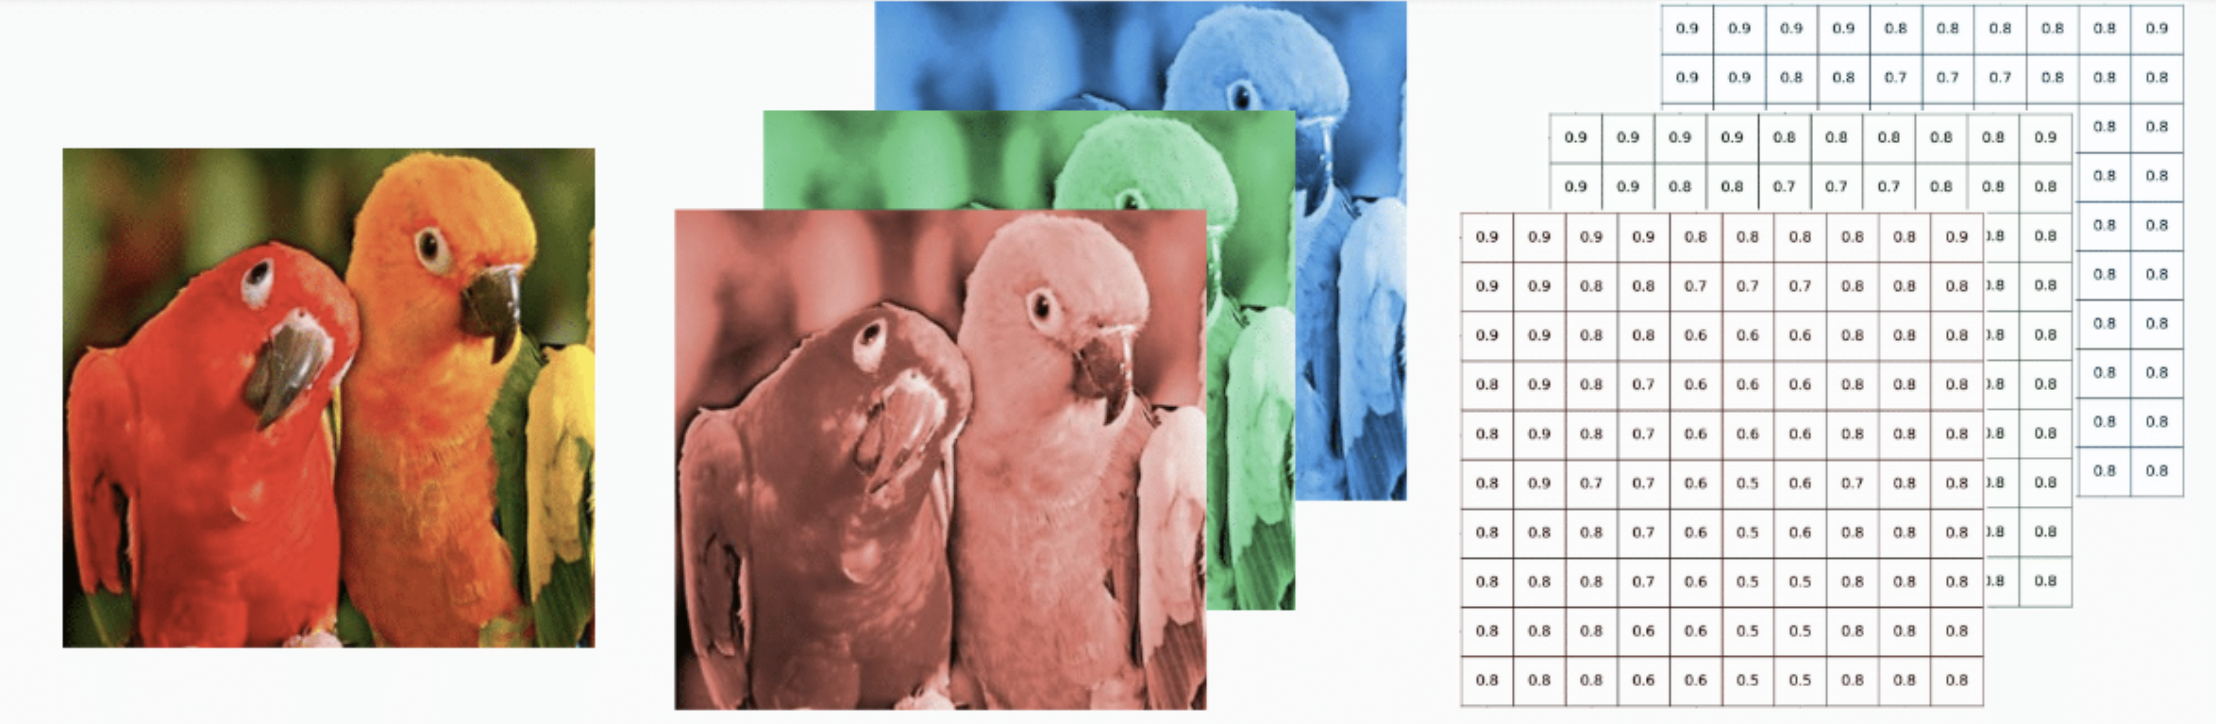
\includegraphics[width=0.9\textwidth]{img/rgbparrot.png}
    \caption{Stacking RGB layers forms final picture}
\end{figure}
\end{frame}

\begin{frame}{Representing Color}
\begin{figure}
    \centering
    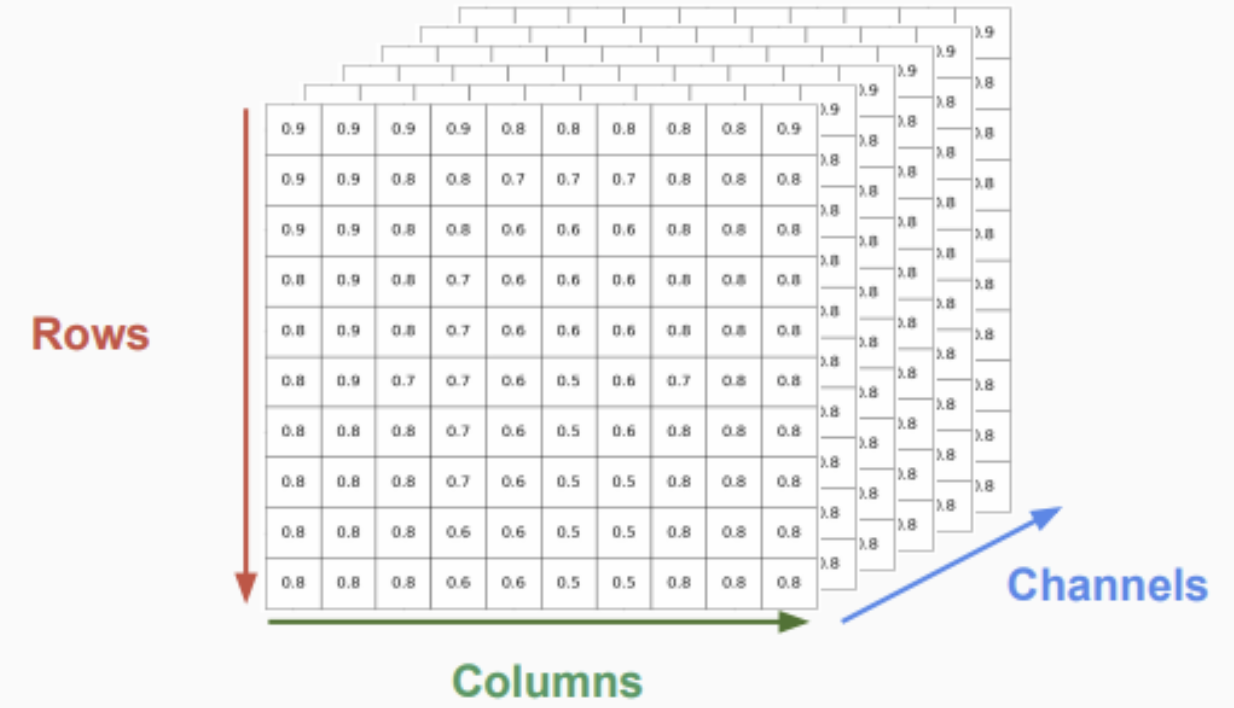
\includegraphics[width=0.7\textwidth]{img/rowcolchannel.png}
    \caption{Numerically, images are 3-dimensional matrices with rows, columns, and 3 \textbf{channels}. We also call these \textbf{volumes}.}
\end{figure}
\end{frame}